% ============================================================
% SIRCA-RAG — Springer LNCS (English version)
% WAIMLAp 2026 / ACSAR
% ============================================================
\documentclass[runningheads]{llncs}

\usepackage[utf8]{inputenc}
\usepackage[T1]{fontenc}
\usepackage[english]{babel}
\usepackage{amsmath,amssymb}
\usepackage{graphicx}
\usepackage{booktabs}
\usepackage{multirow}
\usepackage{array}
\usepackage{enumitem}
\usepackage{url}
\usepackage[dvipsnames]{xcolor}
\usepackage{tikz}
\usetikzlibrary{shapes.geometric,arrows.meta,positioning,calc}
\usepackage[colorlinks=true,
            linkcolor=blue!70!black,
            citecolor=blue!70!black,
            urlcolor=blue!60!black]{hyperref}

\graphicspath{{figures/}}

\newcommand{\sirca}{\textsc{SIRCA-RAG}}

% ============================================================
\title{Hybrid Corrective RAG for Grounded Generation
on Peruvian Medicinal Plants}

\titlerunning{Hybrid Corrective RAG for Peruvian Medicinal Plants}

\author{Ower Lopez-Arela\orcidID{0009-0008-1075-4275} \and
Daniel Marron-Carcausto\orcidID{0009-0008-5964-0201} \and
Antonio Arroyo-Paz\orcidID{0000-0003-1838-4527}}

\authorrunning{O. Lopez-Arela, D. Marron-Carcausto, A. Arroyo-Paz}

\institute{Escuela Profesional de Ingenier\'{i}a de Sistemas, Universidad Nacional de San Agust\'{i}n de Arequipa, Peru\\
\email{\{olopeza, dmarron, aarroyop\}@unsa.edu.pe}}

% ============================================================
\begin{document}
\sloppy
\maketitle

% ============================================================
\begin{abstract}
The vast existing literature on Peruvian medicinal plants suffers from a serious fragmentation problem. Being scattered across numerous repositories, extracting real pharmacological evidence is costly. To address this, we propose \sirca{} (System for Intelligent Retrieval and Corrective Answers), a bilingual architecture designed to unify this evidence through corrective techniques. Our solution fuses dense and lexical (BM25) search using \emph{Reciprocal Rank Fusion}, then applies a cross-encoder reranker that turns out to be vital for protecting answer accuracy. A CRAG-style router manages final quality. We evaluate the tool in a real-world setting with 16{,}486 articles (covering 100 local species), achieving a Fidelity of $0{,}566$ and an MRR of $0{,}837$. On Context Recall — the only metric reported by the comparable prior work — we surpass its result by $18{,}0\%$ relative. We also empirically demonstrate that default normalization ruins routing decisions; we had to force an absolute sigmoid calibration for the derivations toward external search to work legitimately.

\keywords{Retrieval-Augmented Generation (RAG) \and Peruvian Ethnobotany \and Large Language Models (LLM) \and Hybrid Retrieval \and Natural Language Processing (NLP)}
\end{abstract}

% ============================================================
\section{Introduction}
\label{sec:intro}

We know that Peru has around 25{,}000 plant species, and at least between 1{,}400 and 5{,}000 have some degree of pharmacological evidence~\cite{bussmann2006traditional,bussmann2011toxicity}. However, if a researcher wants to track down specific data about \textit{Uncaria tomentosa} or \textit{Croton lechleri}, they will soon run into the central problem: the data is not in one place. Publications are scattered across all of PubMed, as well as local biodiversity databases and international records~\cite{lock2016bioactive,gonzales2012ethnobiology}. Putting together a systematic review under these conditions takes too long and leaves gaps.

Lately, Large Language Models (\emph{LLMs}) have attracted interest for summarizing large volumes of text. By injecting context through Retrieval-Augmented Generation (RAG)~\cite{lewis2020retrieval}, the model appears to ``know'' the subject. In medical practice, however, this hits a wall: the system often pulls in paragraphs that are useless and, worse, invents pharmacological conclusions that look true but lack support~\cite{gao2024retrieval,ji2023survey}. Not even models trained specifically on medical text are spared from this~\cite{lee2020biobert,gu2021domain}. To get around this obstacle, Yan et al.~\cite{yan2024crag} published Corrective RAG (CRAG). The idea behind CRAG is simple but effective: measure whether what you just retrieved is actually useful; if it is not, the model asks to rewrite the query or goes to search the web.

The central contribution we present here is \sirca{} (System for Intelligent Retrieval and Corrective Answers). What we did was take that CRAG concept and adapt it to handle the enormous botanical complexity of Peru. We had to make four strong design decisions. First, we decided not to marry a single retrieval method; we combined \texttt{multilingual-e5-base} vectors~\cite{wang2024e5} with classic BM25 keyword search~\cite{robertson2009bm25} using RRF~\cite{cormack2009rrf}. Second, we added a \emph{cross-encoder}~\cite{nogueira2019passage} because we realized that basic bi-encoders skip over subtle technical details. Third, we implemented a routing safeguard: if confidence drops, we block the generator. Fourth, we forced the model (via CoT~\cite{wei2022chain}) to extract the data, verify it, and only then write the answer, indicating which passage it used. All of this left us with five specific contributions: a bilingual QA architecture for our flora; a massive curated corpus of 16{,}486 articles spanning 100 species; 50 questions we validated ourselves; a way of measuring fidelity that combines lexical with semantic matching; and finally, direct tests with multiple models.

% ============================================================
\section{Related Work}
\label{sec:related}

\textbf{RAG Ecosystem.} It all started with Lewis et al.~\cite{lewis2020retrieval}, who showed that giving a model documents improves what it generates. Years later, Gao et al.~\cite{gao2024retrieval} mapped out all the variants that had emerged since. Of all of them, the proposal by Yan et al.~\cite{yan2024crag} caught our attention for its corrective approach: measuring quality before generating. We took that route, but instead of training an evaluator from scratch, we use the \emph{logits} of a \emph{cross-encoder} directly. There is also Self-RAG~\cite{asai2024selfrag}, which has the LLM decide when it needs more data by generating special tokens, but it requires modifying the LLM internally, which is outside our resource budget.

\textbf{Hybrid Retrieval.} There is enough evidence that mixing dense and sparse approaches works better than using them separately~\cite{karpukhin2020dense}. That is why we chose RRF~\cite{cormack2009rrf} to combine \texttt{e5-base}~\cite{wang2024e5} with BM25~\cite{robertson2009bm25}. The good thing about this is that it does not require labeled data to calibrate weights. Afterward, we simply pass the result to a \emph{cross-encoder}~\cite{nogueira2019passage}.

\textbf{How We Evaluate.} We use the RAGAs framework~\cite{es2023ragas} because it is already a standard. We also added an \emph{LLM-as-judge} mechanism~\cite{zheng2023mtbench} (detailed in Sec.~\ref{sec:llm_judge}) to have a kind of independent cross-audit.

\textbf{The Local Medical Domain.} Xiong et al.~\cite{xiong2024mirage}, with their MIRAGE project, had already shown us that RAG beats raw models on medical topics. Looking at the Latin American level, Monroy Barrios et al.~\cite{monroy2026finetuning} took texts on Peruvian flora and fine-tuned a model directly; they lowered perplexity drastically, but the knowledge stays stuck inside the model's neurons. We prefer RAG because if something goes wrong, we can trace the original document, something vital when we are talking about pharmacology. As a performance reference, Collanqui et al.~\cite{collanqui2026cagrag} achieved a \emph{Recall} of $0{,}417$ with Llama 3.1 on Peruvian law texts, a number we use to compare ourselves against (we reach $0{,}492$). We searched exhaustively and no one had put together a CRAG pipeline with hybrid retrieval for Andean medicinal plants.

% ============================================================
\section{System Architecture}
\label{sec:architecture}

\sirca{} runs five sequential steps per query, orchestrated in Python with FastAPI and LangGraph (Fig.~\ref{fig:architecture}).

\begin{figure}[!ht]
  \centering
  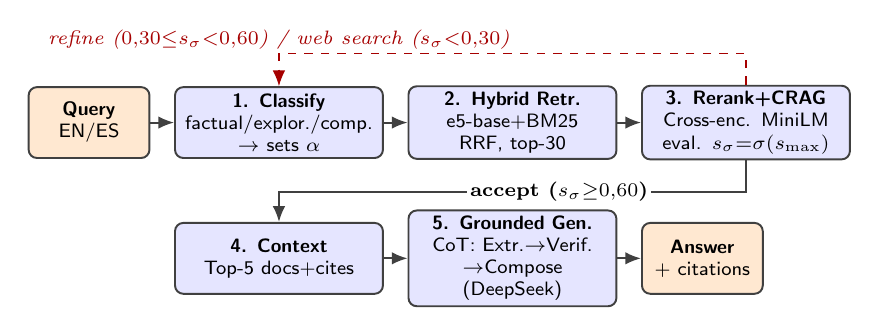
\begin{tikzpicture}[
    font=\sffamily\scriptsize,
    >={Latex[length=2mm,width=1.6mm]},
    phase/.style={rectangle, rounded corners=3pt, draw=black!75, line width=0.7pt,
      minimum height=9mm, text width=25mm, align=center, fill=blue!10, inner sep=2pt},
    io/.style={rectangle, rounded corners=3pt, draw=black!75, line width=0.7pt,
      fill=orange!18, minimum height=9mm, text width=13mm, align=center},
    flow/.style={->, line width=0.7pt, draw=black!75},
    branch/.style={->, line width=0.5pt, draw=red!65!black, dashed},
    blab/.style={font=\scriptsize\itshape, text=red!65!black, fill=white, inner sep=1pt}
  ]
  \node[io] (query) at (0,0) {\textbf{Query}\\{\scriptsize EN/ES}};
  \node[phase, right=3mm of query] (cls)
    {\textbf{1. Classify}\\{\scriptsize factual/explor./comp.}\\{\scriptsize $\rightarrow$ sets $\alpha$}};
  \node[phase, right=3mm of cls] (hyb)
    {\textbf{2. Hybrid Retr.}\\{\scriptsize e5-base+BM25}\\{\scriptsize RRF, top-30}};
  \node[phase, right=3mm of hyb] (crag)
    {\textbf{3. Rerank+CRAG}\\{\scriptsize Cross-enc. MiniLM}\\{\scriptsize eval. $s_{\sigma}{=}\sigma(s_{\max})$}};
  \draw[flow] (query)--(cls); \draw[flow] (cls)--(hyb); \draw[flow] (hyb)--(crag);
  \node[phase, below=8mm of cls.south, anchor=north] (ctx)
    {\textbf{4. Context}\\{\scriptsize Top-5 docs+cites}};
  \node[phase, right=3mm of ctx] (gen)
    {\textbf{5. Grounded Gen.}\\{\scriptsize CoT: Extr.$\rightarrow$Verif.}\\{\scriptsize $\rightarrow$Compose (DeepSeek)}};
  \node[io, right=3mm of gen] (ans) {\textbf{Answer}\\{\scriptsize + citations}};
  \draw[flow] (ctx)--(gen); \draw[flow] (gen)--(ans);
  \draw[flow] (crag.south)--++(0,-4mm)-|(ctx.north)
    node[pos=0.2, font=\scriptsize\bfseries, fill=white, inner sep=1pt]{accept ($s_{\sigma}{\geq}0{,}60$)};
  \draw[branch] (crag.north)--++(0,4mm)-|(cls.north)
    node[pos=0.5, blab, anchor=south]{refine ($0{,}30{\leq}s_{\sigma}{<}0{,}60$) / web search ($s_{\sigma}{<}0{,}30$)};
  \end{tikzpicture}
  \caption{\sirca{}'s five-phase pipeline. Classification sets $\alpha$; hybrid retrieval uses RRF; cross-encoder reranking feeds the CRAG router; and grounded generation applies Chain-of-Thought. Dashed arrows mark CRAG's corrective routes.}
  \label{fig:architecture}
\end{figure}

The full process is split into phases connected to one another. The first thing the system does is read the question and decide what type of query it is. Depending on the verbal patterns we find, we bucket it as \textit{factual}, \textit{exploratory}, or \textit{comparative}. This classification is not mere decoration; it internally alters the weight $\alpha$ we give to retrieval. If we are asked for a hard fact, we give more weight to BM25 keyword matching ($\alpha{=}0{,}3$). If the question is open-ended, we favor the semantic side ($\alpha{=}0{,}7$).

Once classification is done, parallel retrieval kicks in. On one track runs \texttt{multilingual-e5-base}~\cite{wang2024e5}, turning the text into 768-dimensional vectors that are compared mathematically in FAISS~\cite{johnson2021billion}. On the other track runs BM25~\cite{robertson2009bm25}, searching for specific terms the vector might have missed. Both result lists collide and interleave through a simple positional formula called RRF~\cite{cormack2009rrf}, leaving us with a basket of 30 candidate texts.

That is where \texttt{ms-marco-MiniLM-L-12-v2}~\cite{nogueira2019passage} comes into play. This module takes the 30 texts and the original question, and reads them together to refine the relevance score. We keep only the top 10. At this point, the system evaluates the maximum score obtained. We pass that score through a sigmoid function to flatten it and decide: if it exceeds $0{,}60$ (and the rest of the documents are not deficient), we approve the batch. If it falls between $0{,}30$ and $0{,}60$, we raise a ``refinement'' alert. And if it is below $0{,}30$, the system gives up on its local database and emits the signal to fall back to the internet. In the next section we explain why this mathematical decision to use the sigmoid turned out to be vital for the design.

Finally, if the batch was approved, we take the top 5 excerpts and pass them to the DeepSeek V4-Flash model~\cite{deepseek2026v4}\footnote{Accessed through the official DeepSeek API (\url{https://api.deepseek.com}), under the model identifier \texttt{deepseek-v4-flash}.}. We do not simply demand the answer outright; we impose a logical flow of extracting, comparing, and only then drafting. And most critically: its ability to infer data not present in those paragraphs is explicitly blocked.

% ============================================================
\section{Corpus and Evaluation}
\label{sec:experiments}

\textbf{On the data handled.} We combed through eight large repositories to compile this. We reviewed PubMed, Europe PMC, Semantic Scholar, and CrossRef, in addition to hard databases such as GBIF, PeruNPDB, WFO, and COCONUT. We focused on 100 plants from southern Peru. We removed all duplicate articles by cross-checking DOIs and ended up with 16{,}486 unique documents. We split all that text into 512-word chunks (with some overlap so as not to cut ideas in half). Ninety-one of those plants did have literature; the rest (\textit{Adesmia spinosissima}, \textit{Berberis lutea}, among other high-altitude flowers) yielded practically nothing useful. We document this on purpose to test how the system fails later on. We have published this entire corpus online for anyone who wants to review it.

\textbf{On the experiments.} We ourselves created a set of 50 questions in Spanish and English (mixing concept questions, comparisons, and hard facts) about 12 species, and validated what the ideal answer should be. To avoid relying on that alone, we set up the evaluation on three fronts: the 50 base questions; an extended set covering 30 additional species to see whether the system gets dizzy; and a batch of questions we designed maliciously to force the system to fail and trigger the web rescue.

As for how we measure success, we follow standard parameters. On the retrieval side we use Context Precision, Recall, MRR, and NDCG. On the generation side, we use BERTScore F1~\cite{zhang2020bertscore}. And to make sure the model is not hallucinating medical data, we devised a ``Fidelity'' metric that blends semantic evaluation with literal text matches. We also ran simulations removing pieces of the system step by step (what we call ablation) to test what happened.

% ============================================================
\section{Results}
\label{sec:results}

Table~\ref{tab:baselines} shows how \sirca{} compares against the closest published system under the same RAGAs framework for Spanish-language biomedical and normative text. The improvement in Context Recall is $18{,}0\%$ in relative terms ($7{,}5$ absolute percentage points: $0{,}492$ versus $0{,}417$) over Collanqui et al.~\cite{collanqui2026cagrag}; it is worth noting that this quantitative comparison applies only to Context Recall, since that prior work does not report MRR or Fidelity (``---'' cells in Table~\ref{tab:baselines}). The MRR of $0{,}837$ indicates that, for the large majority of queries, the most relevant document lands in the first or second rank position.

\begin{table}[!ht]
\centering
\caption{Comparison against the closest published baseline under the RAGAs framework. ``---'' = metric not reported.}
\label{tab:baselines}
\footnotesize
\begin{tabular}{l l c c c}
\toprule
\textbf{System} & \textbf{LLM} & \textbf{C.Recall} & \textbf{MRR} & \textbf{Fidel.} \\
\midrule
Collanqui et al.~\cite{collanqui2026cagrag} (CAG) & Llama 3.1 & 0{,}417 & --- & --- \\
\textbf{\sirca{} (ours)} & DeepSeek V4-Flash & \textbf{0{,}492} & \textbf{0{,}837} & \textbf{0{,}566} \\
\bottomrule
\end{tabular}
\end{table}

Generation metrics are also solid: BERTScore F1 of $0{,}841$ (\texttt{roberta-large}), Semantic Similarity of $0{,}852$, and Answer Relevancy of $0{,}998$. The exception is Entity Coverage ($0{,}402$), which lags behind the rest. We manually inspected what was going on with the queries that scored lowest. We discovered that the generator's final step is extremely selective: it tends to mention a single compound or plant per statement (whichever has the most textual support) and ignores secondary entities that do appear in the reference paragraph. As a result, automated metrics that demand entity exhaustiveness penalize it, even though the answer is technically correct. Fidelity of $0{,}566$, in turn, reflects the effect of the 35\% lexical component: that factor deliberately penalizes paraphrasing of chemical formulas and taxonomic names to reduce the risk of pharmacological hallucination.

\begin{table}[!ht]
\centering
\caption{Retrieval metrics (top-30 pool, hybrid RRF + cross-encoder, same methodology as Table~\ref{tab:full_results}) over the initial subset ($n{=}12$ human-verified species) and an extension of 30 additional species sampled from the catalog (42 unique species in total).}
\label{tab:extended_retrieval}
\resizebox{0.9\linewidth}{!}{%
\begin{tabular}{l c c c c c c}
\toprule
\textbf{Subset} & $n_{\text{spp}}$ & \textbf{MRR} & \textbf{NDCG@5} & \textbf{NDCG@10} & \textbf{C.\ Precision} & \textbf{C.\ Recall} \\
\midrule
Initial human-verified & 12 & $0{,}837$ & $0{,}757$ & $0{,}750$ & $0{,}415$ & $0{,}492$ \\
Extension (30 new species) & 30 & $0{,}870$ & $0{,}816$ & $0{,}841$ & $0{,}463$ & $0{,}535$ \\
\bottomrule
\end{tabular}%
}
\end{table}

\textbf{Retrieval generalization.} Table~\ref{tab:extended_retrieval} shows that retrieval quality holds up — and in fact improves slightly — when the evaluation scope is widened to 30 unseen species from the corpus: on that set MRR rises from $0{,}837$ to $0{,}870$, NDCG@10 rises from $0{,}750$ to $0{,}841$, and Context Recall also improves ($0{,}492 \rightarrow 0{,}535$). We do not interpret this as evidence that the 30 new species are inherently easier, but rather as confirmation that the retrieval engine is not overfit to the 12 human-verified species subset: it generalizes to unseen data without degradation.

\subsection{Robustness Across Multiple Models}
\label{sec:multi_llm}

The question arose of whether what we observed was an artifact exclusive to the DeepSeek model. To rule this out, we swapped the engine and set up Cerebras Gemma-4-31B~\cite{googledeepmind2026gemma4} to answer the same 50 questions. The retrieval numbers did not change, since they occur earlier in the chain, but the writing did — measurably so (Table~\ref{tab:multi_llm}).

\begin{table}[!ht]
\centering
\caption{Empirical comparison of the generator engine (DeepSeek V4-Flash vs. Cerebras Gemma-4-31B) keeping the \sirca{} pipeline fixed. Paired $t$-tests.}
\label{tab:multi_llm}
\resizebox{0.9\linewidth}{!}{%
\begin{tabular}{l c c c l}
\toprule
\textbf{Metric} & \textbf{DeepSeek-V4} & \textbf{Gemma-4-31B} & $\Delta$ & \textbf{Significance (paired $t$)} \\
\midrule
BERTScore F1          & $0{,}841$ & $0{,}830$ & $-0{,}011$ & \textbf{Significant} ($p{=}0{,}005$) \\
Semantic Similarity & $0{,}852$ & $0{,}789$ & $-0{,}063$ & Not significant ($p{=}0{,}18$) \\
Entity Coverage& $0{,}402$ & $0{,}386$ & $-0{,}016$ & Not significant ($p{=}0{,}46$) \\
Relevancy            & $0{,}998$ & $0{,}988$ & $-0{,}010$ & \textbf{Significant} ($p{=}0{,}042$) \\
\midrule
\textbf{Fidelity} (hybrid) & $0{,}517$ & $\mathbf{0{,}609}$ & $\mathbf{+0{,}092}$ & \textbf{Significant} ($p{<}0{,}001$) \\
\bottomrule
\end{tabular}%
}
\end{table}

The results show a more nuanced pattern than we anticipated: DeepSeek V4-Flash matches or beats Gemma-4-31B on four of the five generation metrics — including BERTScore F1 ($p{=}0{,}005$) and Relevancy ($p{=}0{,}042$), both significant in DeepSeek's favor — while Semantic Similarity and Entity Coverage show no significant differences. The only metric where Gemma is clearly superior is Fidelity ($p{<}0{,}001$). We attribute this single advantage to Gemma's more literal compositional style, which tends to reproduce scientific names and phrases from the context almost verbatim — which specifically benefits the lexical component (35\,\%) of our hybrid Fidelity — while on general quality metrics (BERTScore, Relevancy) DeepSeek's more fluent writing is not penalized. The architecturally relevant point is twofold: (i)~the \sirca{} pipeline tolerates swapping the generator without additional tuning, and (ii)~the choice of generator does matter for Fidelity specifically, not for generation quality in general. Unlike an early run of this same experiment, this run recorded no blank answers from either model ($0/50$ each), following the retry fix described in Limitation~(vii).

\subsection{Cross-Validation}
\label{sec:llm_judge}

We wanted to be sure our Fidelity metric was not lying to us. So we applied the \emph{LLM-as-judge} technique~\cite{zheng2023mtbench}, having Gemma-4 itself rate, on a 0-to-4 scale, how well DeepSeek had answered relative to the texts provided. We deliberately made the evaluator model come from a different family to avoid friendly biases. The qualitative result is encouraging: 43 of the 50 answers scored a perfect 4/4, one scored 3, five scored 2, and a single one received zero for not providing useful information. That $86\%$ of perfect scores, however, leaves very little variance in the judge for a formal correlation: the Pearson coefficient between the judge's score and our algorithmic metric came out low and not significant ($r{=}0{,}056$, $p{=}0{,}70$), expected when one of the two variables is concentrated almost entirely at its maximum value (ceiling effect).

What is interesting here is the raw gap in the numbers. The judge averaged high scores ($0{,}925$ normalized), but our metric was much harsher ($0{,}517$). This happened because we designed our formula to be unforgiving toward medical paraphrasing: we would rather have the system report a low score than validate a phrase that ``sounds similar'' but could contain a clinical error. We acknowledge that no artificial judge will replace the toxicological rigor of a human pharmacist; the exercise works better as a coarse qualitative filter (detecting unsupported answers) than as a strict quantitative validation of Fidelity, given the ceiling effect observed.

\begin{table}[!ht]
\centering
\caption{Ablation of six configurations (50 queries). Retrieval: agent-based methodology with the sigmoid-calibrated CRAG evaluator (script \texttt{run\_perquery\_agent\_ablation.py}). Fidelity: reported for \texttt{full} and \texttt{no\_reranker} with DeepSeek V4-Flash generation (script \texttt{run\_n5\_fidelity\_wilcoxon.py}); ``n/a'' denotes configurations whose per-query LLM re-run remains future work (Limitation iii). Bold = best; underline = worst per column. $^\dagger$\texttt{dense\_only} matches \texttt{full} on retrieval because after reranking the Top-10 is identical across all 50 queries (invariant to $\alpha$ once the cross-encoder dominates); \texttt{no\_classifier} does \textbf{not} share that invariance (see Section~\ref{sec:wilcoxon}).}
\label{tab:full_results}
\footnotesize
\begin{tabular}{l c c c c c c}
\toprule
\textbf{Config.} & \textbf{C.Prec.} & \textbf{C.Recall} & \textbf{MRR} & \textbf{NDCG@10} & \textbf{Fidel.} & $\boldsymbol{\Delta}$\textbf{Fidel.} \\
\midrule+
\texttt{full}           & 0{,}411 & 0{,}482 & 0{,}825 & 0{,}741 & \textbf{0{,}566} & --- \\
\texttt{dense\_only}$^\dagger$ & 0{,}411 & 0{,}482 & 0{,}825 & 0{,}741 & n/a & n/a \\
\texttt{sparse\_only}   & \underline{0{,}402} & \underline{0{,}466} & \underline{0{,}752} & \underline{0{,}666} & n/a & n/a \\
\texttt{no\_reranker}   & 0{,}418 & 0{,}476 & \textbf{0{,}869} & 0{,}751 & \underline{0{,}465} & $-17{,}8\%$ \\
\texttt{no\_crag}       & 0{,}431 & 0{,}511 & 0{,}851 & 0{,}772 & n/a & n/a \\
\texttt{no\_classifier} & \textbf{0{,}479} & \textbf{0{,}558} & 0{,}862 & \textbf{0{,}833} & n/a & n/a \\
\bottomrule
\end{tabular}
\end{table}

\subsection{Findings from Taking the System Apart}

Removing pieces one by one (Table~\ref{tab:full_results}) revealed four uncomfortable but useful truths. First, the reranking module is literally the system's shield. When we turned it off, Fidelity dropped by $17{,}8\%$ relative (from $0{,}566$ to $0{,}465$), a statistically significant difference by paired Wilcoxon ($p{=}0{,}00023$; Sec.~\ref{sec:wilcoxon}). It turns out the initial fusion does bring relevant texts to the top of the list, but they come accompanied by ``false friends'' that end up misleading the generator if the reranker does not filter them out in time. Second, keyword search alone (\texttt{sparse\_only}) turned out to be the weakest configuration on all four retrieval metrics (C.Prec. $0{,}402$, C.Recall $0{,}466$, MRR $0{,}752$, NDCG@10 $0{,}666$, all the worst value per column): without the dense component, BM25 loses the synonyms and wording variants across the 50 queries. Third, and even more uncomfortable: disabling the query classifier (\texttt{no\_classifier}) \emph{improves} retrieval significantly relative to \texttt{full} — C.Prec. $+16{,}5\%$ ($p{=}0{,}007$), C.Recall $+15{,}8\%$ ($p{<}0{,}001$), and NDCG@10 $+12{,}4\%$ ($p{=}0{,}003$) — suggesting that the classifier's per-category fixed $\alpha$ ($0{,}3$/$0{,}7$/$0{,}5$) is worse calibrated than a fixed compromise of $\alpha{=}0{,}6$ for this benchmark; we discuss this tension in Section~\ref{sec:wilcoxon}. Fourth, \texttt{dense\_only} does produce exactly the same Top-10 as \texttt{full} across all 50 queries ($n_{\neq}{=}0$): once the cross-encoder reranks, the initial bias toward pure dense retrieval becomes irrelevant. Looking at the clock, retrieval takes us barely $\sim$1\,810\,ms to process on CPU, and drafting takes between 10 and 30 seconds using the DeepSeek server.

\subsection{Statistical Significance of the Ablation Deltas}
\label{sec:wilcoxon}

The differences between configurations in Table~\ref{tab:full_results} are point estimates and could be due to chance. To rule this out, we ran paired Wilcoxon signed-rank tests on the per-query values (50 queries, two-sided test) between each ablation variant and the \texttt{full} configuration. Table~\ref{tab:wilcoxon} summarizes the $p$-values for Context Precision, Context Recall, MRR, and NDCG@10.

\begin{table}[!ht]
\centering
\caption{Wilcoxon signed-rank $p$-values (two-sided) against \texttt{full}, computed on per-query retrieval metrics using the same agent-based methodology as Table~\ref{tab:full_results}. The significance test on Fidelity is reported separately for the central \texttt{full} vs \texttt{no\_reranker} comparison (two paragraphs below, $p{=}0{,}00023$; script \texttt{run\_n5\_fidelity\_wilcoxon.py}); extending it to all six configurations requires re-running the LLM for each one and remains future work. ``---'' denotes configurations whose retrieved Top-10 is identical to \texttt{full} ($n_{\neq}{=}0$ across all four metrics). $n_{\neq}$ = number of queries with a non-zero difference in the C.Recall column (each metric has its own $n_{\neq}$; C.Recall's is reported as a reference).}
\label{tab:wilcoxon}
\footnotesize
\begin{tabular}{l c c c c c}
\toprule
\textbf{Config.} & \textbf{$n_{\neq}$} & \textbf{C.Prec.} & \textbf{C.Recall} & \textbf{MRR} & \textbf{NDCG@10} \\
\midrule
\texttt{dense\_only}    &  0 & --- & --- & --- & --- \\
\texttt{sparse\_only}   & 40 & 0{,}450 & 0{,}523 & 0{,}241 & 0{,}100 \\
\texttt{no\_reranker}   & 24 & 0{,}637 & 0{,}786 & 0{,}345 & 0{,}695 \\
\texttt{no\_crag}       &  5 & 0{,}043 & 0{,}043 & 0{,}068 & 0{,}043 \\
\texttt{no\_classifier} & 20 & \textbf{0{,}007} & \textbf{0{,}0004} & 0{,}307 & \textbf{0{,}003} \\
\bottomrule
\end{tabular}
\end{table}

The statistical picture forces us to slow down. \texttt{sparse\_only} not only has the lowest aggregate Recall ($0{,}466$ versus $0{,}482$ for \texttt{full}); the difference also fails to reach significance at the per-query level ($p{=}0{,}523$ on C.Recall, $n_{\neq}{=}40$): BM25 without the dense component loses on some queries and wins on others, and the net effect is indistinguishable from chance despite being consistently the worst average. \texttt{dense\_only} does produce exactly the same Top-10 as \texttt{full} ($n_{\neq}{=}0$, marked with ``---''): the cross-encoder reranker makes final retrieval indifferent to which $\alpha$ the fusion started from. The finding that breaks intuition is \texttt{no\_classifier}: unlike \texttt{dense\_only}, there is a real and \emph{significant} difference against \texttt{full} here on three of four metrics (C.Prec. $p{=}0{,}007$, C.Recall $p{<}0{,}001$, NDCG@10 $p{=}0{,}003$; MRR not significant, $p{=}0{,}307$), and in the opposite direction from what would be expected: using a fixed $\alpha$ of $0{,}6$ for every query retrieves better than the per-category $\alpha$ the classifier assigns. This does not invalidate the classifier's usefulness for other purposes (e.g., explainability of the routing decision), but it does indicate that its current $\alpha$ calibration ($0{,}3$/$0{,}7$/$0{,}5$ per category) is not optimized for this benchmark and deserves a hyperparameter sweep in future work. \texttt{no\_crag} does differ from \texttt{full}, though in only $5$ of $50$ queries according to C.Recall ($p{=}0{,}043$, significant at the $95\%$ level): disabling CRAG means those queries no longer trigger \textsc{refine}/\textsc{web\_search} and the final context the generator receives changes; for the rest of the queries CRAG accepts the same Top-10 in both configurations. The overall reading is that, at the retrieval level, the ablation does reveal real and in some cases counterintuitive differences — not all configurations are statistically equivalent — but the most consistent and architecturally central impact of the ablation still lives in Fidelity, where removing the reranker costs a $-17{,}8\%$ relative drop (Table~\ref{tab:full_results}), a generation metric that the retrieval tests fail to capture. To verify that this drop is not noise, we applied a paired Wilcoxon signed-rank test on per-query Fidelity between \texttt{full} and \texttt{no\_reranker} (with DeepSeek generation): the difference is statistically significant ($p{=}0{,}00023$ two-sided; $p{=}0{,}00012$ one-sided, with all 50/50 queries registering a non-zero difference). That is, unlike some retrieval metrics, the reranker's contribution to Fidelity — the article's central claim — does robustly clear the significance test.

\textbf{Note on runs and the absolute value of Fidelity.} DeepSeek's Fidelity in the cross-LLM comparison (Table~\ref{tab:multi_llm}, $0{,}517$) differs from \texttt{full}'s Fidelity in Table~\ref{tab:full_results} ($0{,}566$) because they come from different runs of the commercial API: Table~\ref{tab:multi_llm} uses the paired run with Gemma-4, while Table~\ref{tab:full_results} uses a dedicated ablation run. The one result reproducible across runs — and the one that supports the article's conclusion — is the \emph{direction} and \emph{significance} of the differences, not the absolute value of the metrics.

\subsection{The Normalization Trap}
\label{sec:crag_validation}

We ran into a huge technical obstacle halfway through. The evaluation tool we were using had the habit of stretching each text block's scores from $0$ to $1$. This means that, even if every retrieved text was garbage, the ``least bad'' one received a perfect $1{,}0$. As a result, the system gave a green light to everything and never activated the external rescue searches. We had to step into the architecture and calibrate the raw numbers using an absolute sigmoid curve. We set the margins at $0{,}60$ to approve and $0{,}30$ to doubt. That fixed the problem at the root.

To prove this actually worked, we threw an arsenal of 27 trap questions at the system. Some were about plants we knew were not in the database; others were computing-world absurdities like ``Vue.js''; and others were simply disconnected words. Table~\ref{tab:crag_stress} shows how the algorithm defended itself.

\begin{table}[!ht]
\centering
\caption{System decisions when processing 27 stress queries. Family A: taxa with no indexed data; Family B: topics outside the botanical domain; Family C: degraded lexical strings.}
\label{tab:crag_stress}
\footnotesize
\begin{tabular}{l c c c c}
\toprule
\textbf{Family} & $n$ & \textbf{\textsc{accept}} & \textbf{\textsc{refine}} & \textbf{\textsc{web\_search}} \\
\midrule
A. Species with no data & 9 & 1 & 3 & 5 \\
B. Off-domain   & 10 & 0 & 0 & \textbf{10} \\
C. Garbled           &  8 & 4 & 0 & 4 \\
\midrule
Total (\emph{probes})            & 27 & 5 & 3 & 19 \\
Total (in-domain \emph{benchmark}) & 50 & 35 & 5 & 10 \\
\bottomrule
\end{tabular}
\end{table}

The observed behavior matched theoretical expectations. Faced with off-topic subjects, the system redirected to external search $100\%$ of the time. When asked about plants absent from the corpus, in $8$ of $9$ attempts it requested reformulating the premise or reached out to the internet. There was a single bypass with \textit{Senecio canescens}, caused by the engine retrieving data from phylogenetically related taxa. On the in-domain benchmark itself (50 queries), the absolute calibration does not always yield \textsc{accept}: $35/50$ route to \textsc{accept}, $5/50$ to \textsc{refine}, and $10/50$ to \textsc{web\_search}. We interpret these $15$ corrective activations as correct behavior rather than false negatives: they are disproportionately concentrated in \textit{exploratory} and \textit{comparative} queries ($12/15$, $80\%$, versus $51\%$ among accepted queries), categories that by design call for synthesis across multiple sources rather than a single fact, and are therefore more prone to genuinely ambiguous retrieval. We prefer the system to declare uncertainty in those cases rather than fabricate an answer. In short, we empirically demonstrate that the redirection mechanism works successfully and that, by replacing intra-batch normalization with absolute sigmoid calibration, the corrective route activates both on out-of-distribution inputs and on low-confidence in-domain queries — the previous normalization bug had suppressed this second case, making it indistinguishable from nominal behavior.

% ============================================================
\section{Discussion}
\label{sec:discussion}

When processing herbal-medicine queries, we face heterogeneous structures. A user might ask for ``common names'' while concatenating a rigorous academic term such as \textit{Uncaria tomentosa}. As we document, lexical search is unbeatable for capturing Latin names, but the hybrid method is justified because the \emph{cross-encoder} steps in to weed out results that lack semantic cohesion. Additionally, natively handling multiple languages through the vector space mitigated considerable computational barriers.

Looking at other efforts, such as the team of Monroy Barrios et al.~\cite{monroy2026finetuning}, they forcibly injected Andean texts into Llama's brain. That gives fluent answers, but if a doctor asks you where you got that dosage from, there is no way to prove it. Our path with RAG keeps the data outside, auditable, with a traceable reference number. We believe the obvious future lies in merging both worlds: fine-tuning a model and, on top of that, adding a protective RAG layer.

\textbf{Availability and limitations.} The complete code is published at \url{https://github.com/yughiyami/rag_medicinal_plants}; there is also an interactive demo at \url{https://rag.scn.quest} where the retrieved fragments with their DOI/PMID and the CRAG routing decision for each query can be observed in real time. We list below the current limitations so readers can correctly gauge the scope of the results: (i)~the human-verified \emph{benchmark} covers 12 of the 100 species in the corpus; retrieval was verified on 42 species in total (Sec.~\ref{sec:results}) and routing on the 9 species with no indexed data (Sec.~\ref{sec:crag_validation}), but full answer-quality evaluation over the remaining 58 species requires building additional reference answers; (ii)~current reference answers were authored by the authors themselves; although the Fidelity metric was cross-checked against an independent LLM-judge (Sec.~\ref{sec:llm_judge}), validation by an external pharmacognosy or ethnobotany specialist is still pending, and that is the first requirement before any clinical or production use; (iii)~we tested significance on Fidelity for the central comparison (\texttt{full} vs \texttt{no\_reranker}, $p{=}0{,}00023$; Sec.~\ref{sec:wilcoxon}); extending the Fidelity test to all six ablation configurations requires re-running the LLM for each one and remains future work; (iv)~hybrid Fidelity (65\% semantic + 35\% lexical) was cross-checked against an LLM-judge in Sec.~\ref{sec:llm_judge}; the judge's $86\%$ rate of perfect scores serves as a coarse qualitative filter, but the formal correlation was not significant due to the resulting ceiling effect ($r{=}0{,}056$, $p{=}0{,}70$), so this validation should be read as indicative rather than as quantitative proof; correlation with expert human judgments remains an open research question; (v)~robustness across LLMs was verified with a second generator (Cerebras Gemma-4-31B); extending that verification to other families (Llama, Qwen, Mistral) would strengthen the generality claim; (vi)~the calibration thresholds ($\sigma_{\mathrm{acc}}{=}0{,}60$, $\sigma_{\mathrm{ref}}{=}0{,}30$) come from the cross-encoder's sigmoid curve and were validated on 27 \emph{probes}; a systematic sweep over a broader OOD set would allow fine-tuning the operating point; (vii)~an early run of the cross-LLM evaluation (Sec.~\ref{sec:multi_llm}) showed the DeepSeek V4-Flash generator returning blank or truncated answers on $8/50$ queries ($16\%$); we diagnosed the cause (no retry on empty content in the HTTP client) and fixed it with retry and exponential backoff, which eliminated the problem entirely ($0/50$ in the run reported in this article); we keep a record of the original finding because it could resurface with other API providers that fail similarly; (viii)~absolute values of the generation metrics depend on the point in time at which the commercial DeepSeek API was accessed, so exact reproduction may differ from the values reported here; the directional and significance conclusions are stable across runs.

% ============================================================
\section{Conclusions}
\label{sec:conclusion}

Throughout this manuscript we outlined \sirca{}'s architecture. We integrated parallel retrieval methods, incorporated a strict reranker, established absolute mathematical calibration safeguards, and forced the model to use sequential reasoning before synthesizing bilingual botanical outputs. After subjecting the system to the corpus of 100 Peruvian healing species, the metrics were conclusive: we surpass the Context Recall of previous approaches implemented for this regional framework by $18{,}0\%$ relative. We empirically confirmed that the reranker is the most critical link in the trust chain; removing it reduces Fidelity in a statistically significant way ($-17{,}8\%$ relative, $p{=}0{,}00023$). Cross-validation tests with a second generator (Cerebras Gemma-4-31B) confirmed that the architecture tolerates swapping the LLM without design changes, although three of the five generation metrics — Fidelity, BERTScore F1, and Relevancy — do vary in a statistically significant way depending on the chosen generator. We observed firsthand how standard software's default behaviors compromise corrective pipelines if one does not intervene directly in the mechanics of empirical normalization. As a corollary, the future trajectory is clear: it is imperative to set up panels with biologists to audit the answers under strict professional scrutiny~\cite{heinrich2020ethnopharmacology}, extend the scope of our geographic tests, and, on a more ambitious scale, run parametric modifications on the LLM's weights to internalize botanical ontology prior to document analysis.

% ============================================================

% ============================================================
\bibliographystyle{splncs04}
\bibliography{references}

\end{document}
